\chapter{Results and Future Work}\label{chapter:Conclusion}
\section{Result}
In the case of the gradient descent algorithm, the interpolation conditons for $m$-$L$ sector bounded functions and $m$-strong $L$-smooth convex functions are the same. Therefore, to see if the \texttt{AlgorithmAnalysis.jl} package is able to analyze the gradient descent algorithm over the $m$-$L$ sector bounded function class, we can plot the rate bound of this case and compare it with the analysis results of the same algorithm and step size but for $m$-strong $L$-smooth convex functions presented in Figure 2 of \cite{tutorial}. In order to produce comparable results, we run the analysis 19 $m$-$L$ value pairs where the condition number $L/m$ varies between 1 and 100. The code used to produce this analysis result is presented in Figure~\ref{ex_tested_result}. The convergence rate guarantee found for each condition number is shown in Figure~\ref{plot_result}.
\begin{figure}[h!]
	\begin{lstlisting}[mathescape]
m, condnum, = 1, [range(1,10,10); range(20,100,9)]
# condition numbers tested
GDresults = []
for L in condnum
    # Stop if the algorithm doesn't converge
    if length(GD) > 0 && last(GD) == 1
        append!(GD, 1)
    else
        $\alpha$ = 2/(L+m)
        @algorithm begin
            f = DifferentiableFunctional{R$^n$}()
            xs = first_order_stationary_point(f)
            f' $\in$ SectorBounded(m, L, xs, f'(xs))
            x0 = R$^n$()
            x1 = x0 - $\alpha$*f'(x0)
            x0 => x1
            performance = (x0-xs)^2
        end
        append!(GD, rate(performance))
    end
end
plot(condnum, [GD], title="", label="GD", xaxis=:log)
xlabel!("Condition number L/m")
ylabel!("Convergence rate bound")
\end{lstlisting}
\caption{Analysis results for GD and $m$-$L$ sector bounded functions over 19 $L/m$ condition numbers}
\label{ex_tested_result}
\end{figure}
% \begin{code}{julia}{A sample code listing. The method \texttt{rate} performs the automated algorithm analysis by searching for a Lyapunov function that bounds the rate of convergence of the performance measure.}{code:label}
%     m,L = 1,10                                   # parameters
%     α = 2/(L+m)                                  # stepsize
    
%     @algorithm begin
%       f = DifferentiableFunctional{Rⁿ}()       # objective function
%       xs = first_order_stationary_point(f)     # first-order stationary point
%       f' ∈ SectorBounded(m, L, xs, f'(xs))     # function class
%       x0 = Rⁿ()                                # initial point
%       x1 = x0 - α*f'(x0)                       # gradient descent
%       x0 => x1                                 # state update
%       performance = (x1-xs)^2                  # performance measure
%     end
    
%     rate(performance)                            # automated algorithm analysis
%     \end{code}
\begin{figure}[h]
    \centering
    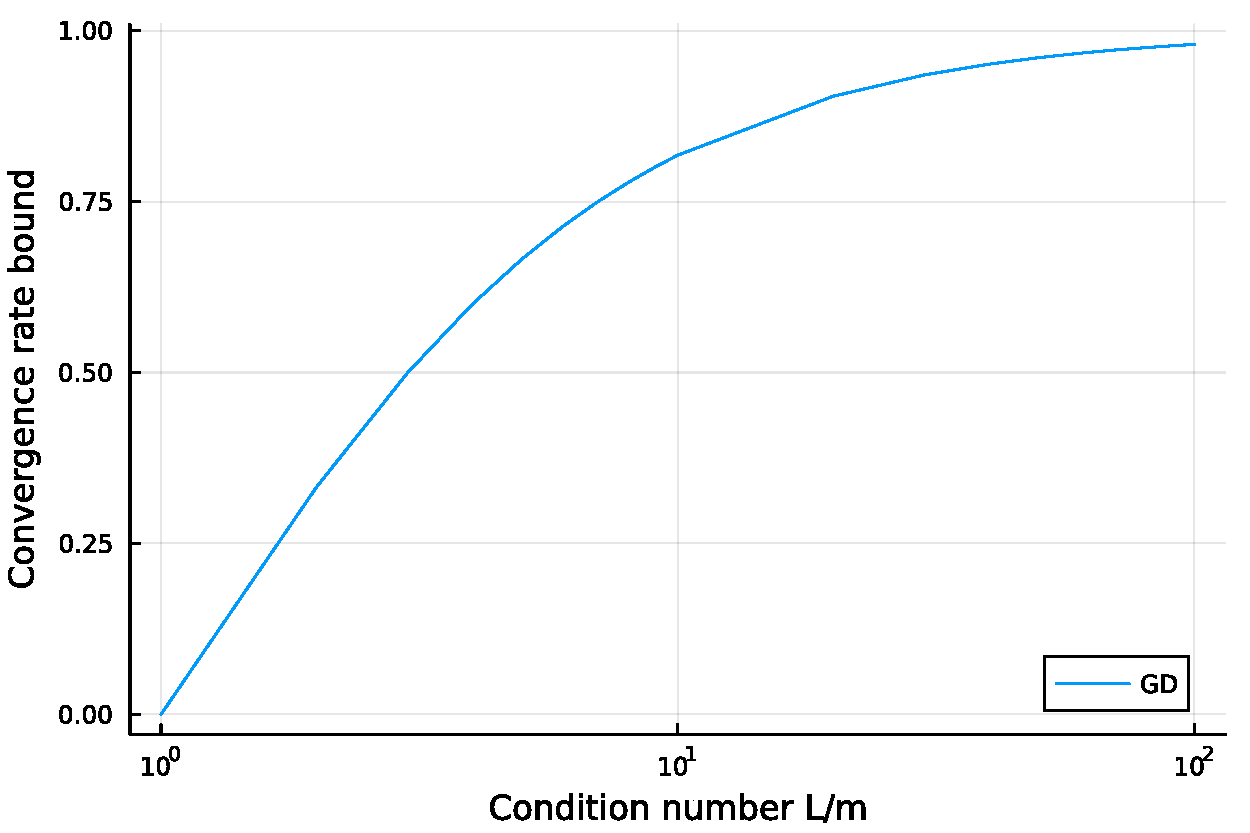
\includegraphics[width = .8 \textwidth]{plot.pdf}
    \caption{Convergence rate guarantee of gradient descent at optimizing $1-10$ sector bounded functions}
    \label{plot_result}
\end{figure}

\section{Future work}
Following this thesis proposal, the future work include finish coding the program. While most to all of the package have been coded, the program is only able to produce result correctly matching the analysis result produced in \cite{tutorial} for the gradient descent algorithm. As a result, the program need to be debugged and tested to ensure it is able to correctly implement the mathematical approach to algorithm analysis and produce accurate results.

Additionally, the program currently does not support ''lifting dimension'', an optional step of the Lyapunov method to algorithm analysis in \cite{tutorial}. Part of the future work of this research work is to implement this step and measure its effect on the tightness of the convergence rate guarantee.

A crucial step before the package can be completed and delivered as end-user software and part of the future work of this thesis is the documentation of Algorithm Analysis, which includes writing operating instructions, providinig analysis examples, detailing the package's components, and the steps the program takes to perform algorithm analysis.